%%%%%%%%%%%%%%%%%%%%%%%%%%%%%%%%%%%%%%%%%
%
% Optics and Radar -based observations
% Assignment 2
%
%%%%%%%%%%%%%%%%%%%%%%%%%%%%%%%%%%%%%%%%%

%----------------------------------------------------------------------------------------
%	DOCUMENT CONFIGURATIONS
%----------------------------------------------------------------------------------------

\documentclass{article}

\title{\textbf {Optics and Radar Based Observations} \\ Assignment 2\\ Pulse Modulation Techniques} % Title

\def\authors{
Ivan \v Sinkarenko\\
Anuraj Rajendraprakash
}
\author{\authors}

\usepackage{graphicx}
\usepackage{fullpage}

% load package with ``framed'' and ``numbered'' option.
\usepackage[framed,numbered,autolinebreaks,useliterate]{mcode}

\begin{document}

\maketitle % Insert the title, author and date

\centerline{Referee: Dr. Anita Enmark}

%\vspace{10mm}
%\begin{figure}[h!]
%\centering
%\centerline{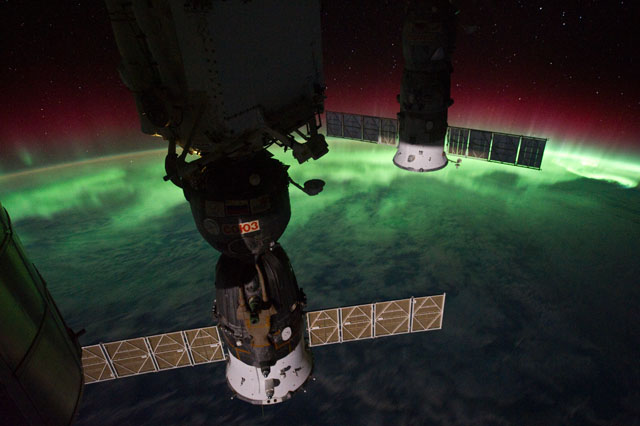
\includegraphics[width=\textwidth]{Figures/iss.jpg}}
%\label{fig:iss}
%\end{figure}

\setlength\parindent{0pt} % Removes all indentation from paragraphs

\renewcommand{\labelenumi}{\alph{enumi}.} % Make numbering in the enumerate environment by letter rather than number (e.g. section 6)
\clearpage

\tableofcontents

\listoffigures

\clearpage

%----------------------------------------------------------------------------------------
%	SECTION 1. Introduction
%----------------------------------------------------------------------------------------

\section{Introduction}
MST (mesosphere-stratosphere-troposphere) radars are applied to study winds, waves, turbulence and in- stability in the atmosphere. They usually operate near 50 MHz and also called VHF radars (VHF-very high frequency band between 30 MHz and 300 MHz).\\
\\
ESRAD (ESrange RADar) is VHF MST radar located in northern Sweden (6756N, 2104E). It has been in near continuous operation since June 1996. The purpose of the radar is to provide information on the dynamic state of the atmosphere - winds, waves, turbulence and layering from the troposphere up to the lower thermosphere (1 km -100 km altitude). ESRAD operates at a frequency of 52 MHz corresponding to a wavelength of 5.77 m. The transmitter consists of 72 1-kW solid-state modules that are grouped into 12 6-kW power blocks. The resulting peak power output power is 72 kW and the maximum duty cycle is 5\%. Pulse repetition frequency rates from 100 Hz to 16 kHz are possible. Pulse lengths correspond to height resolutions between 150 m and 3 km. The radar is capable of pulse coding the transmitted signals using both Barker and complementary codes. The radar has 6 separate receivers for detection of backscattered signals from the atmosphere. The complex (in-phase and quadrature) data samples are recorded using a 12-channel data acquisition unit. The bandwidth of the separate receiving elements is 2 MHz. Multiple receivers allows post-detection beam-steering and full spectral analysis of the returned signal. The digital processing system is able to process up to 256 heights per sample and integrates up to 4096 pulse repetitions per sample. The antenna consists of a 12 x 12 phased array of 5-element Yagis, each being approximately 6 m high. The Yagis are spaced about 4 m apart (corresponding to 0.7 times the radar wavelength). \cite{Enmark:2012a2}
 
%----------------------------------------------------------------------------------------
%	SECTION 2. Part 1
%----------------------------------------------------------------------------------------

\section{Part 1}

In pulsed radar and sonar signal processing, an ambiguity function is a two-dimensional function of time delay and Doppler frequency $\chi(\tau,f)$ showing the distortion of a returned pulse due to the receiver matched filter[1] (commonly, but not exclusively, used in pulse compression radar) due to the Doppler shift of the return from a moving target. The ambiguity function is determined by the properties of the pulse and the matched filter, and not any particular target scenario.

Autocorrelation is the cross-correlation of a signal with itself. Informally, it is the similarity between observations as a function of the time separation between them. It is a mathematical tool for finding repeating patterns, such as the presence of a periodic signal which has been buried under noise, or identifying the missing fundamental frequency in a signal implied by its harmonic frequencies. It is often used in signal processing for analysing functions or series of values, such as time domain signals.

In order to have high range resolutions, the use of short pulses is important in radar applications. However there are several limitations to the use of short pulses. The bandwidth of a short pulse is large because the bandwidth is inversely proportional to the pulse width. A large bandwidth of the signal makes the radar system complex, places greater demand on the signal processing and increases the chances of interference with other electromagnetic signals. A large bandwidth also reduces the dynamic range of the receiver because the noise power is proportional to the bandwidth. Also the short pulses don't have high resolution in the doppler frequency measurement. Short pulses also places more demands on transmitter peak power. 

Pulse compression is a technique which allows the radar to simultaneously achieve the energy of a long pulse and the resolution of a short pulse by avoiding the use of high peak power which is needed in high energy short duration pulse. In this method a long pulse is made to have the same bandwidth as a short pulse by modulation it in frequency or phase.

\begin{figure}[htb]
\begin{minipage}[t]{0.5\linewidth}
\centering
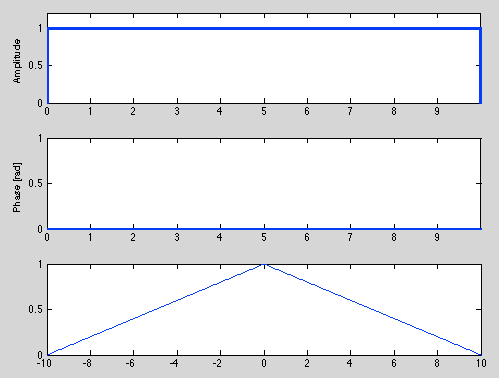
\includegraphics[width=8cm]{Figures/long_pulse_data.png}
\caption{Auto-correlation function of a long pulse.}
\label{fig:long_pulse_data}
\end{minipage}
%\hspace{0.5cm}
\begin{minipage}[t]{0.5\linewidth}
\centering
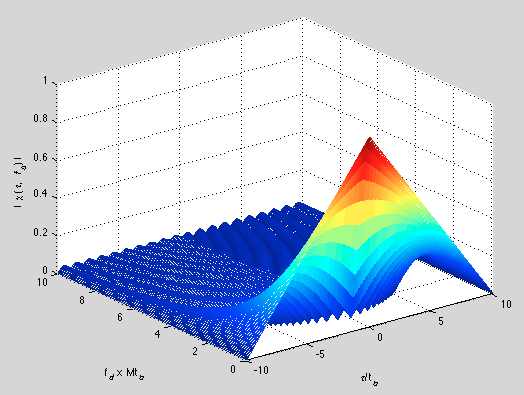
\includegraphics[width=8cm]{Figures/long_pulse_3d.png}
\caption{Ambiguity function of a long pulse.}
\label{fig:long_pulse_3d}
\end{minipage}
\end{figure}

\begin{figure}[htb]
\begin{minipage}[t]{0.5\linewidth}
\centering
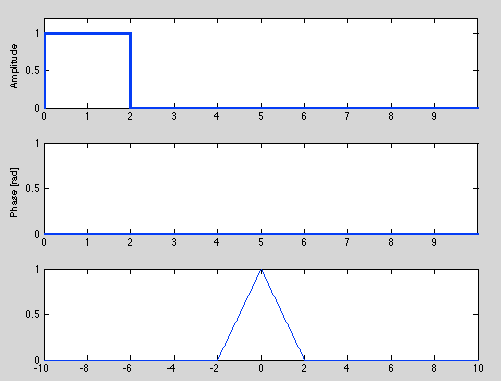
\includegraphics[width=8cm]{Figures/short_pulse_data.png}
\caption{Auto-correlation function of a short pulse.}
\label{fig:short_pulse_data}
\end{minipage}
%\hspace{0.5cm}
\begin{minipage}[t]{0.5\linewidth}
\centering
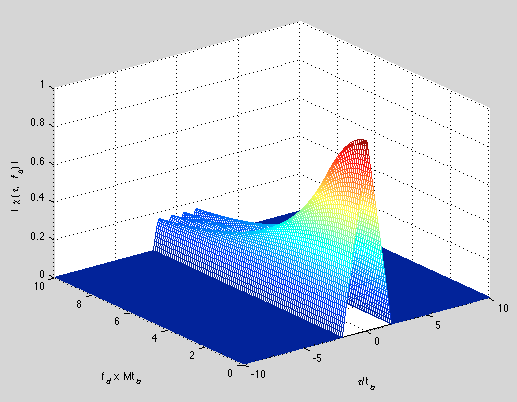
\includegraphics[width=8cm]{Figures/short_pulse_3d.png}
\caption{Ambiguity function of a short pulse.}
\label{fig:short_pulse_3d}
\end{minipage}
\end{figure}

Figure \ref{fig:long_pulse_data} and Figure \ref{fig:long_pulse_3d} show the autocorrelation and ambiguity function of a long pulse. For a square pulse response is centered around origin. There is no response outside the the width $\tau$, which is observed both in the autocorrelation and ambiguity function plots. The time delay measurement error is proportinal to the pulse width and the frequency measurement error is proportional to the inverse of the pulse width. Thus the frequency measurement accuracy for a long pulse would be good while the time delay measurement accuracy would be worse. \cite{Skolnik:2001irs}

\begin{figure}[htb]
\begin{minipage}[t]{0.5\linewidth}
\centering
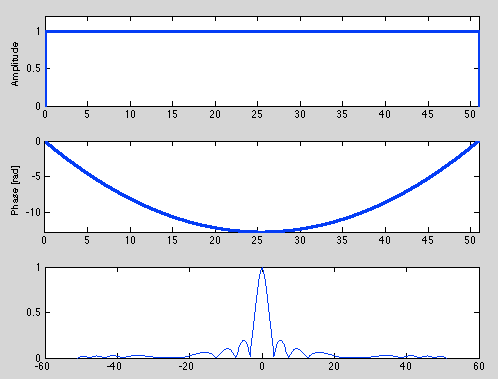
\includegraphics[width=8cm]{Figures/lfm_data.png}
\caption{Auto-correlation function of frequency coding with LFM.}
\label{fig:lfm_data}
\end{minipage}
%\hspace{0.5cm}
\begin{minipage}[t]{0.5\linewidth}
\centering
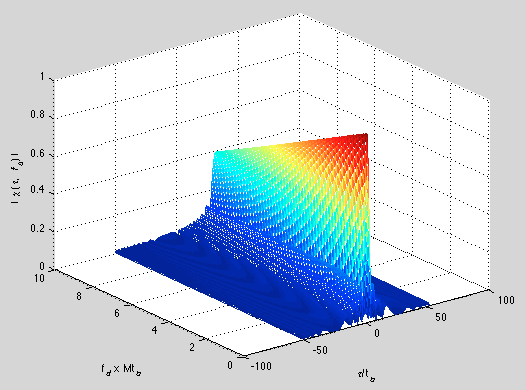
\includegraphics[width=8cm]{Figures/lfm_3d.png}
\caption{Ambiguity function of frequency coding with LFM.}
\label{fig:lfm_3d}
\end{minipage}
\end{figure}

Figure \ref{fig:short_pulse_data} and Figure \ref{fig:short_pulse_3d} show the autocorrelation and ambiguity function of a short pulse. As it can be seen in Figure \ref{fig:short_pulse_data} and Figure \ref{fig:short_pulse_3d}, the response is centered around origin. There is no response outside the the pulse width $\tau$. Thus the frequency measurement accuracy for a long pulse would be worse while the time delay measurement accuracy would be good. \cite{Skolnik:2001irs}

The Figure \ref{fig:lfm_data} and Figure \ref{fig:lfm_3d} show the auto correlation and ambiguity function of the Linear Frequency Modulated(LFM) signal. In such a signal the time delay measurement accuracy is proportional to the inverse of the bandwidth and the frequency measurement accuracy is proportional to inverse of the pulse width.  The pulse width and the bandwidth are independant of each other and hence the time delay and frequency measurement accuracy are also independent of each other.

\begin{figure}[htb]
\begin{minipage}[t]{0.5\linewidth}
\centering
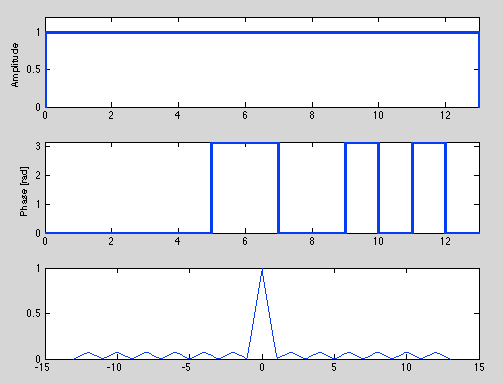
\includegraphics[width=8cm]{Figures/barker_data.png}
\caption{Auto-correlation function of Barker coding (13).}
\label{fig:barker_data}
\end{minipage}
%\hspace{0.5cm}
\begin{minipage}[t]{0.5\linewidth}
\centering
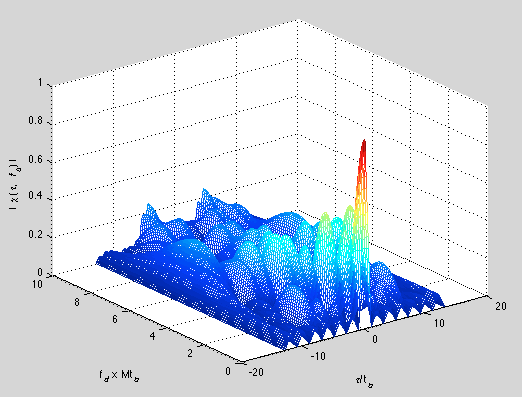
\includegraphics[width=8cm]{Figures/barker_3d.png}
\caption{Ambiguity function of Barker coding (13).}
\label{fig:barker_3d}
\end{minipage}
\end{figure}

The Figure \ref{fig:barker_data} and Figure \ref{fig:barker_3d} show the auto correlation and the ambiguity function plots of a long pulse compressed by barker coding. One of the ways of increasing the bandwidth of a long pulse for the purpose of pulse compression, is by changing the phase. A long pulse of duration T is divided in to N subpulses of width $\tau$. The bandwidth is increased by changing the phase of each subpulse. A common form of phase change is \textit{binary phase coding}, in which the phases are made either 0 or $\pi$ according to a specified criterion. If the 0 and $\pi$ phase selection are made at random then the time side lobes have higher magnitude. Barker codes are a set sequences of 0 and $\pi$ phases for the subpulses so that the side lobes have lower side lobe levels. If the barker codes are used for the phases of the subpulses then all the time side lobes have equal magnitude. \cite{Skolnik:2001irs}. This is clearly observed in the Figures \ref{fig:barker_data} and \ref{fig:barker_3d}.

\begin{figure}[htb]
\begin{minipage}[t]{0.5\linewidth}
\centering
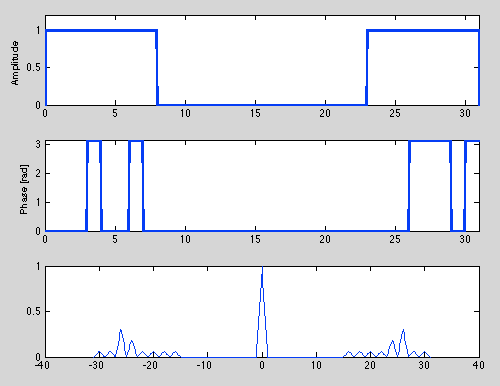
\includegraphics[width=8cm]{Figures/complementary_data.png}
\caption{Auto-correlation function of complementary coding (7).}
\label{fig:complementary_data}
\end{minipage}
%\hspace{0.5cm}
\begin{minipage}[t]{0.5\linewidth}
\centering
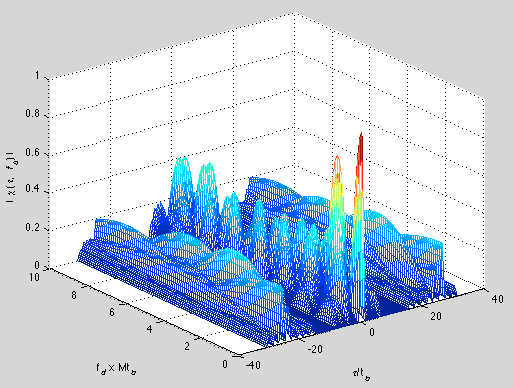
\includegraphics[width=8cm]{Figures/complementary_3d.png}
\caption{Ambiguity function of complementary coding (7).}
\label{fig:complementary_3d}
\end{minipage}
\end{figure}

The auto correlation and the ambiguity function plot of a long pulse compressed with complementary coding is shown in Figure \ref{fig:complementary_data} and Figure \ref{fig:complementary_3d} respectively. Using the complementary codes for the phase selections is another method of achieving pulse compression. In this coding method, pairs of equal length phase-coded pulses are chosen so that the side lobes of the auto correlation function of one are the negative of the other. In complemenatary coding  the auto correlation function from the outputs of the two matched filters are added. This results in the algebraic sum of the side lobes being zero and the main response being 2N where N is the number of subpulses.




%----------------------------------------------------------------------------------------
%	SECTION 3. Part 2
%----------------------------------------------------------------------------------------

\section{Part 2}

%----------------------------------------------------------------------------------------
%	SUBSECTION 3.1. Part 2A
%----------------------------------------------------------------------------------------

\subsection{Part 2A}

The height resolution obtainable with atmospheric radar is limited by the need to transmit a pulse of finite length. Since atmospheric properties change significantly within a few 10s a pulse should be as short as possible. However, the strength of the signal obtained from the atmosphere is proportional to the pulse length. Since the signal should be as strong as possible to be easily detectable above the natural noise, the radar pulse should be as long as possible. In practice we must always choose some compromise between these two conflicting demands. \cite{Enmark:2012a2}


\begin{figure}[htb]
\begin{minipage}[t]{0.5\linewidth}
\centering
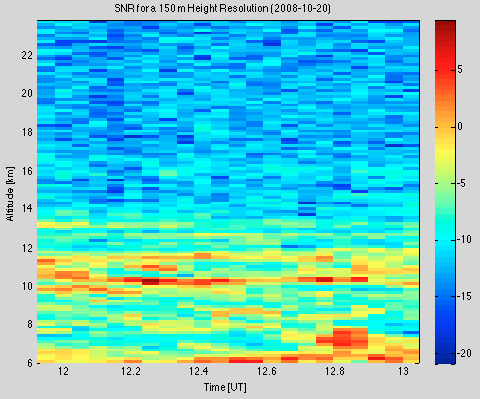
\includegraphics[width=8cm]{Figures/height_res_150m.png}
\caption{SNR data for 150 m height resolution.}
\label{fig:height_res_150m}
\end{minipage}
%\hspace{0.5cm}
\begin{minipage}[t]{0.5\linewidth}
\centering
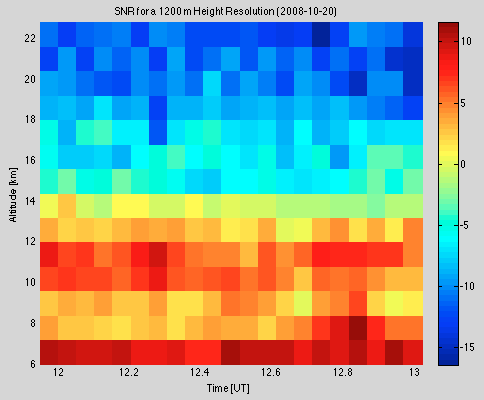
\includegraphics[width=8cm]{Figures/height_res_1200m.png}
\caption{SNR data for 1200 m height resolution.}
\label{fig:height_res_1200m}
\end{minipage}
\end{figure}

%----------------------------------------------------------------------------------------
%	SUBSECTION 3.2. Part 2B
%----------------------------------------------------------------------------------------

\subsection{Part 2B}

\begin{figure}[htb]
\begin{minipage}[t]{0.5\linewidth}
\centering
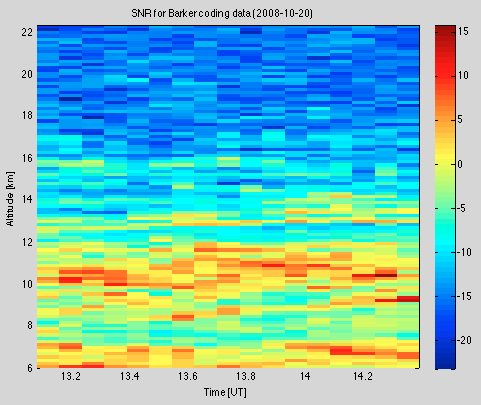
\includegraphics[width=8cm]{Figures/SNR_barker.png}
\caption{SNR for Barker coding data.}
\label{fig:SNR_barker}
\end{minipage}
%\hspace{0.5cm}
\begin{minipage}[t]{0.5\linewidth}
\centering
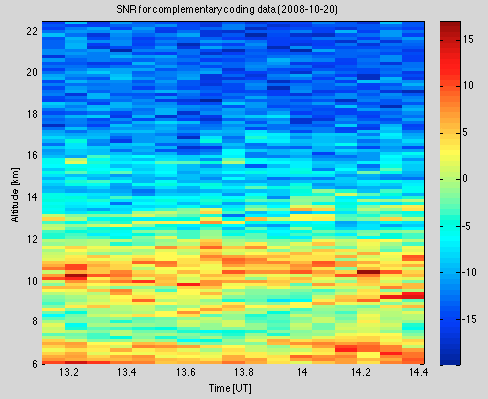
\includegraphics[width=8cm]{Figures/SNR_complementary.png}
\caption{SNR for complementary coding data.}
\label{fig:SNR_complementary}
\end{minipage}
\begin{minipage}[b]{0.5\linewidth}
\vspace{0.5cm}
\centering
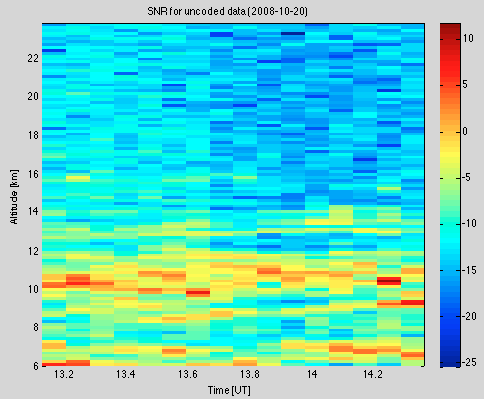
\includegraphics[width=8cm]{Figures/SNR_uncoded.png}
\caption{SNR for uncoded data.}
\label{fig:SNR_uncoded}
\end{minipage}
\end{figure}



\begin{figure}[htb]
\begin{minipage}[t]{0.5\linewidth}
\centering
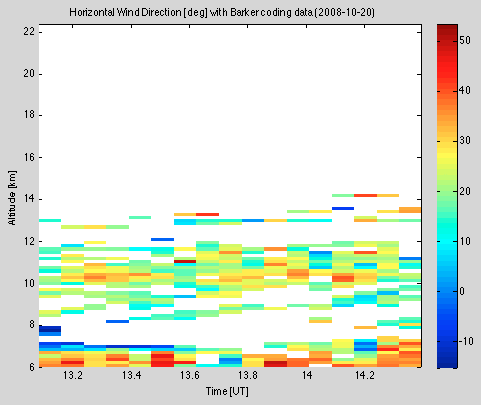
\includegraphics[width=8cm]{Figures/wind_dir_barker.png}
\caption{Horizontal wind direction with Barker coding data.}
\label{fig:wind_dir_barker}
\end{minipage}
\begin{minipage}[t]{0.5\linewidth}
\centering
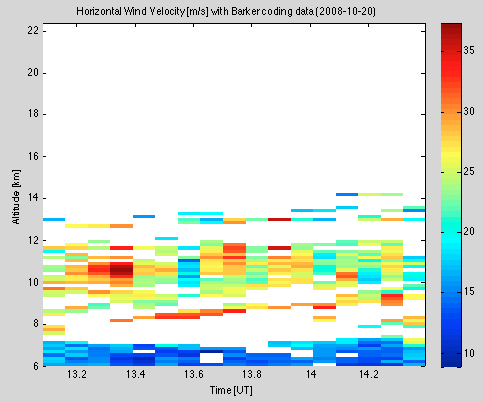
\includegraphics[width=8cm]{Figures/wind_vel_barker.png}
\caption{Horizontal wind velocity with Barker coding data.}
\label{fig:wind_vel_barker}
\end{minipage}
\end{figure}

\begin{figure}[htb]
\begin{minipage}[t]{0.5\linewidth}
\centering
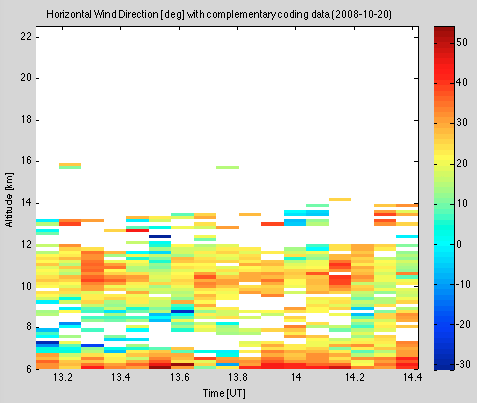
\includegraphics[width=8cm]{Figures/wind_dir_complementary.png}
\caption{Horizontal wind direction with complementary coding data.}
\label{fig:wind_dir_complementary}
\end{minipage}
\begin{minipage}[t]{0.5\linewidth}
\centering
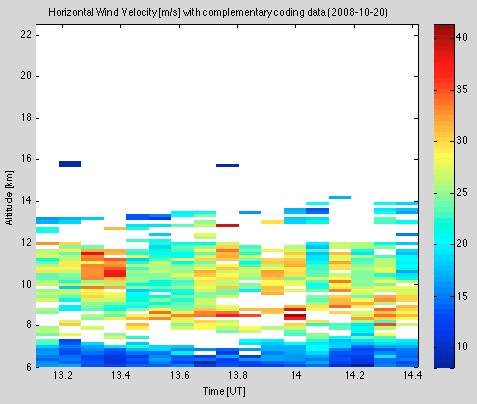
\includegraphics[width=8cm]{Figures/wind_vel_complementary.png}
\caption{Horizontal wind velocity with complementary coding data.}
\label{fig:wind_vel_complementary}
\end{minipage}
\end{figure}

\begin{figure}[htb]
\begin{minipage}[t]{0.5\linewidth}
\centering
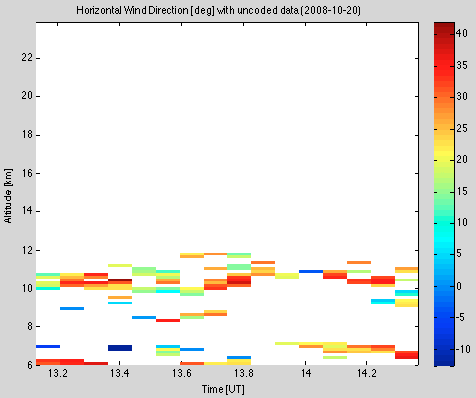
\includegraphics[width=8cm]{Figures/wind_dir_uncoded.png}
\caption{Horizontal wind direction with uncoded data.}
\label{fig:wind_dir_uncoded}
\end{minipage}
\begin{minipage}[t]{0.5\linewidth}
\centering
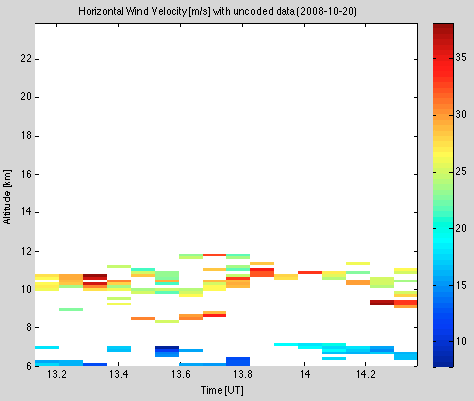
\includegraphics[width=8cm]{Figures/wind_vel_uncoded.png}
\caption{Horizontal wind velocity with uncoded data.}
\label{fig:wind_vel_uncoded}
\end{minipage}
\end{figure}


%----------------------------------------------------------------------------------------
%	SECTION 4. REFERENCES
%----------------------------------------------------------------------------------------

\begin{thebibliography}{9}

\bibitem{Enmark:2012a2}
Enmark A.  (2012).
\newblock {\em Assignment 2. Pulse Modulation Techniques}.
\newblock Lule\aa \ University of Technology, Kiruna, Sweden.

\bibitem{Skolnik:2001irs}
Skolnik M. ~I.  (2001).
\newblock {\em Introduction to Radar Systems}.
\newblock The McGraw-Hill Companies, Inc., New York, United States.

\bibitem{LevanonMozeson:2004rs}
Levanon N. and Mozeson E. (2004).
\newblock {\em Radar Signals}.
\newblock John Wiley \& Sons, Inc., New Jersey, United States.
\end{thebibliography}

%http://www.mathworks.com/matlabcentral/


%----------------------------------------------------------------------------------------
%	SECTION 5. Appendix 2A
%----------------------------------------------------------------------------------------

\section{Appendix 2A. Matlab code of Part 2A}

\subsection{Part2A.m}
\lstinputlisting{Part2A.m}

\subsection{plotSNR.m}
\lstinputlisting{plotSNR.m}

%----------------------------------------------------------------------------------------
%	SECTION 6. Appendix 2B
%----------------------------------------------------------------------------------------

\section{Appendix 2B. Matlab code of Part 2B}

\subsection{Part2B.m}
\lstinputlisting{Part2B.m}

\subsection{plotWind.m}
\lstinputlisting{plotWind.m}

\subsection{hypotenuse.m}
\lstinputlisting{hypotenuse.m}

\subsection{radToDeg.m}
\lstinputlisting{radToDeg.m}

%----------------------------------------------------------------------------------------
%	SECTION 7. Confirmation
%----------------------------------------------------------------------------------------

\section{Acknowledgements}


\end{document}